% Options for packages loaded elsewhere
\PassOptionsToPackage{unicode}{hyperref}
\PassOptionsToPackage{hyphens}{url}
%
\documentclass[
  8pt,
  ignorenonframetext,
  t]{beamer}
\usepackage{pgfpages}
\setbeamertemplate{caption}[numbered]
\setbeamertemplate{caption label separator}{: }
\setbeamercolor{caption name}{fg=normal text.fg}
\beamertemplatenavigationsymbolsempty
% Prevent slide breaks in the middle of a paragraph
\widowpenalties 1 10000
\raggedbottom
\setbeamertemplate{part page}{
  \centering
  \begin{beamercolorbox}[sep=16pt,center]{part title}
    \usebeamerfont{part title}\insertpart\par
  \end{beamercolorbox}
}
\setbeamertemplate{section page}{
  \centering
  \begin{beamercolorbox}[sep=12pt,center]{part title}
    \usebeamerfont{section title}\insertsection\par
  \end{beamercolorbox}
}
\setbeamertemplate{subsection page}{
  \centering
  \begin{beamercolorbox}[sep=8pt,center]{part title}
    \usebeamerfont{subsection title}\insertsubsection\par
  \end{beamercolorbox}
}
\AtBeginPart{
  \frame{\partpage}
}
\AtBeginSection{
  \ifbibliography
  \else
    \frame{\sectionpage}
  \fi
}
\AtBeginSubsection{
  \frame{\subsectionpage}
}
\usepackage{amsmath,amssymb}
\usepackage{lmodern}
\usepackage{iftex}
\ifPDFTeX
  \usepackage[T1]{fontenc}
  \usepackage[utf8]{inputenc}
  \usepackage{textcomp} % provide euro and other symbols
\else % if luatex or xetex
  \usepackage{unicode-math}
  \defaultfontfeatures{Scale=MatchLowercase}
  \defaultfontfeatures[\rmfamily]{Ligatures=TeX,Scale=1}
\fi
% Use upquote if available, for straight quotes in verbatim environments
\IfFileExists{upquote.sty}{\usepackage{upquote}}{}
\IfFileExists{microtype.sty}{% use microtype if available
  \usepackage[]{microtype}
  \UseMicrotypeSet[protrusion]{basicmath} % disable protrusion for tt fonts
}{}
\makeatletter
\@ifundefined{KOMAClassName}{% if non-KOMA class
  \IfFileExists{parskip.sty}{%
    \usepackage{parskip}
  }{% else
    \setlength{\parindent}{0pt}
    \setlength{\parskip}{6pt plus 2pt minus 1pt}}
}{% if KOMA class
  \KOMAoptions{parskip=half}}
\makeatother
\usepackage{xcolor}
\newif\ifbibliography
\setlength{\emergencystretch}{3em} % prevent overfull lines
\providecommand{\tightlist}{%
  \setlength{\itemsep}{0pt}\setlength{\parskip}{0pt}}
\setcounter{secnumdepth}{-\maxdimen} % remove section numbering
% type setting
% ------------------------------------------------------------------------------
\usepackage[german]{babel}     

% fonts
% ------------------------------------------------------------------------------
\usefonttheme{professionalfonts}

% slide title and horizontal line
% ------------------------------------------------------------------------------
\setbeamertemplate{frametitle}{%
    \vskip-30pt \color{black}\large%
    \begin{minipage}[b][23pt]{120mm}%
    \flushleft\insertframetitle%
    \end{minipage}%
}

\setbeamertemplate{headline}										
{
\vskip10pt\hfill\hspace{3.5mm} 										 
\vskip15pt\color{black}\rule{\textwidth}{0.4pt} 					 
}

% slide number
% ---------------------------------------------------------------
\setbeamertemplate{navigation symbols}{}
\setbeamertemplate{footline}
{
\vskip5pt
\vskip2pt
\makebox[123mm]{\hspace{7.5mm}
\hfill Grundlagen der Mathematik und Informatik $\vert$ 
\copyright $ $ 2022 Belinda Fleischmann CC BY-NC-SA 4.0 $\vert$ 
Folie \insertframenumber}
\vskip4pt
}

% block color scheme
% ------------------------------------------------------------------------------
% colors
\definecolor{white}{RGB}{255,255,255}
\definecolor{grey}{RGB}{235,235,235}
\definecolor{lightgrey}{RGB}{245,245,245}
\definecolor{LightBlue}{RGB}{220,220,255}
\definecolor{darkblue}{RGB}{51, 51, 153}

% definitions and theorems
\setbeamercolor{block title}{fg = black, bg = grey}
\setbeamercolor{block body}{fg = black, bg = lightgrey}

% general line spacing 
% ------------------------------------------------------------------------------
\linespread{1.3}

% local line spacing
% ------------------------------------------------------------------------------
\usepackage{setspace}

% colors
% -----------------------------------------------------------------------------
\usepackage{color}

% justified text
% ------------------------------------------------------------------------------
\usepackage{ragged2e}
\usepackage{etoolbox}
\apptocmd{\frame}{}{\justifying}{}

% bullet point lists
% -----------------------------------------------------------------------------
\setbeamertemplate{itemize item}[circle]
\setbeamertemplate{itemize subitem}[circle]
\setbeamertemplate{itemize subsubitem}[circle]
\setbeamercolor{itemize item}{fg = black}
\setbeamercolor{itemize subitem}{fg = black}
\setbeamercolor{itemize subsubitem}{fg = black}
\setbeamercolor{enumerate item}{fg = black}
\setbeamercolor{enumerate subitem}{fg = black}
\setbeamercolor{enumerate subsubitem}{fg = black}
\setbeamerfont{itemize/enumerate body}{}
\setbeamerfont{itemize/enumerate subbody}{size = \normalsize}
\setbeamerfont{itemize/enumerate subsubbody}{size = \normalsize}

% color links
% ------------------------------------------------------------------------------
\usepackage{hyperref}
\definecolor{urls}{RGB}{204,0,0}
\hypersetup{colorlinks, citecolor = darkblue, urlcolor = urls}


% additional math commands
% ------------------------------------------------------------------------------
\usepackage{bm}                                         % bold math symbols
\newcommand{\niton}{\not\owns}

% text highlighting
% ------------------------------------------------------------------------------
\usepackage{soul}
\makeatletter
\let\HL\hl
\renewcommand\hl{%
  \let\set@color\beamerorig@set@color
  \let\reset@color\beamerorig@reset@color
  \HL}
\makeatother

% equation highlighting
% -----------------------------------------------------------------------------
\newcommand{\highlight}[2][yellow]{\mathchoice%
  {\colorbox{#1}{$\displaystyle#2$}}%
  {\colorbox{#1}{$\textstyle#2$}}%
  {\colorbox{#1}{$\scriptstyle#2$}}%
  {\colorbox{#1}{$\scriptscriptstyle#2$}}}%
  
\ifLuaTeX
  \usepackage{selnolig}  % disable illegal ligatures
\fi
\IfFileExists{bookmark.sty}{\usepackage{bookmark}}{\usepackage{hyperref}}
\IfFileExists{xurl.sty}{\usepackage{xurl}}{} % add URL line breaks if available
\urlstyle{same} % disable monospaced font for URLs
\hypersetup{
  hidelinks,
  pdfcreator={LaTeX via pandoc}}

\author{}
\date{\vspace{-2.5em}}

\begin{document}

\begin{frame}[plain]{}
\protect\hypertarget{section}{}
\center

\begin{center}
\includegraphics[width=0.2\linewidth]{../Abbildungen/glmi_otto} \end{center}

\vspace{2mm}

\huge

Grundlagen der Mathematik und Informatik \vspace{6mm}

\Large

Aufbaukurs: Fit für Psychologie WiSe 2022/23

\vspace{12mm}
\normalsize

Belinda Fleischmann

\vspace{3mm}
\scriptsize

Inhalte basieren auf
\href{https://www.ipsy.ovgu.de/Institut/Abteilungen+des+Institutes/Methodenlehre+I+_+Experimentelle+und+Neurowissenschaftliche+Psychologie/Lehre/Wintersemester+2022/Grundlagen+der+Mathematik+und+Informatik.html}{Einführung
in Mathematik und Informatik} von
\href{https://www.ipsy.ovgu.de/Institut/Abteilungen+des+Institutes/Methodenlehre+I+_+Experimentelle+und+Neurowissenschaftliche+Psychologie/Team/Dirk+Ostwald.html}{Dirk
Ostwald}, lizenziert unter
\href{https://creativecommons.org/licenses/by-sa/4.0/deed.de}{CC
BY-NC-SA 4.0}
\end{frame}

\begin{frame}[plain]{}
\protect\hypertarget{section-1}{}
\vfill
\center
\huge

\textcolor{black}{(0) Einführung} \vfill
\end{frame}

\begin{frame}{Fit für Psychologie - Motivation}
\protect\hypertarget{fit-fuxfcr-psychologie---motivation}{}
\setstretch{1.7}

Elementares Basiswissen für die datenanalytischen Module des BSc
Psychologie

\small

\begin{itemize}
\tightlist
\item
  Modul A2 Forschungsmethoden
\item
  Modul B1 Deskriptive Statistik
\item
  Modul B2 Inferenzstatistik
\item
  Modul C2 Computergestützte Datenanalyse
\end{itemize}

\normalsize

Studien- und Prüfungsordnung BSc Psychologie § 4(2) Zulassung zum
Studium

\small

``Studierende, deren Englisch-, EDV- bzw. Mathematikkenntnisse gering
sind, sollten sich vor Aufnahme des Studiums entsprechend
weiterbilden.''

\normalsize

Elementares Basiswissen für die datenanalytischen Module des MSc
Psychologie

\small

\begin{itemize}
\tightlist
\item
  Modul A1 Multivariate Verfahren
\item
  Modul A3 Computergestützte Datenanalyse
\end{itemize}
\end{frame}

\begin{frame}{Lehrstuhl für Methodenlehre I}
\protect\hypertarget{lehrstuhl-fuxfcr-methodenlehre-i}{}
\setstretch{1.7}

\href{https://www.ipsy.ovgu.de/methodenlehre_I-path-980,1404.html}{\textcolor{blue}{Webseite des Lehrstuhls (Lehre, Forschung, Team)}}

\vspace{3mm}

\begin{center}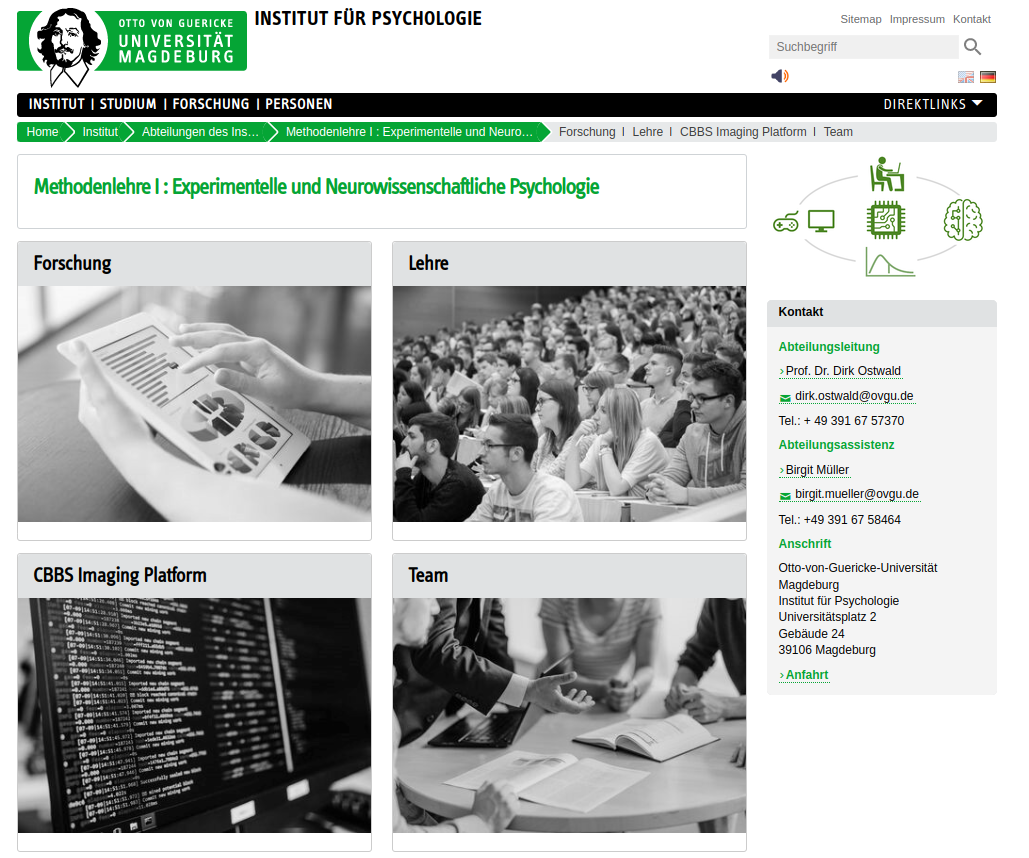
\includegraphics[width=0.7\linewidth]{../Abbildungen/Lehrstuhlseite} \end{center}

\color{red}{TODO}
\end{frame}

\begin{frame}{Fit für Psychologie - Inhalte}
\protect\hypertarget{fit-fuxfcr-psychologie---inhalte}{}
\setstretch{2}
\large
\vfill

\begin{enumerate}
[(1)]
\item
  Mengen
\item
  Summen, Produkte, Potenzen
\end{enumerate}

\textcolor{gray}{(3) Folgen, Reihen, Grenzwerte}

\begin{enumerate}
[(1)]
\setcounter{enumi}{3}
\item
  Funktionen
\item
  Differentialrechnung
\item
  Integralrechnung
\item
  Grundbegriffe der Informatik \vfill
\end{enumerate}
\end{frame}

\begin{frame}{Fit für Psychologie}
\protect\hypertarget{fit-fuxfcr-psychologie}{}
\href{https://www.ipsy.ovgu.de/Institut/Abteilungen+des+Institutes/Methodenlehre+I+_+Experimentelle+und+Neurowissenschaftliche+Psychologie/Lehre/Wintersemester+2022/Grundlagen+der+Mathematik+und+Informatik.html}{\textcolor{blue}{Webseite des Kurses (Folien, Videos)}}

\vspace{5mm}

\begin{center}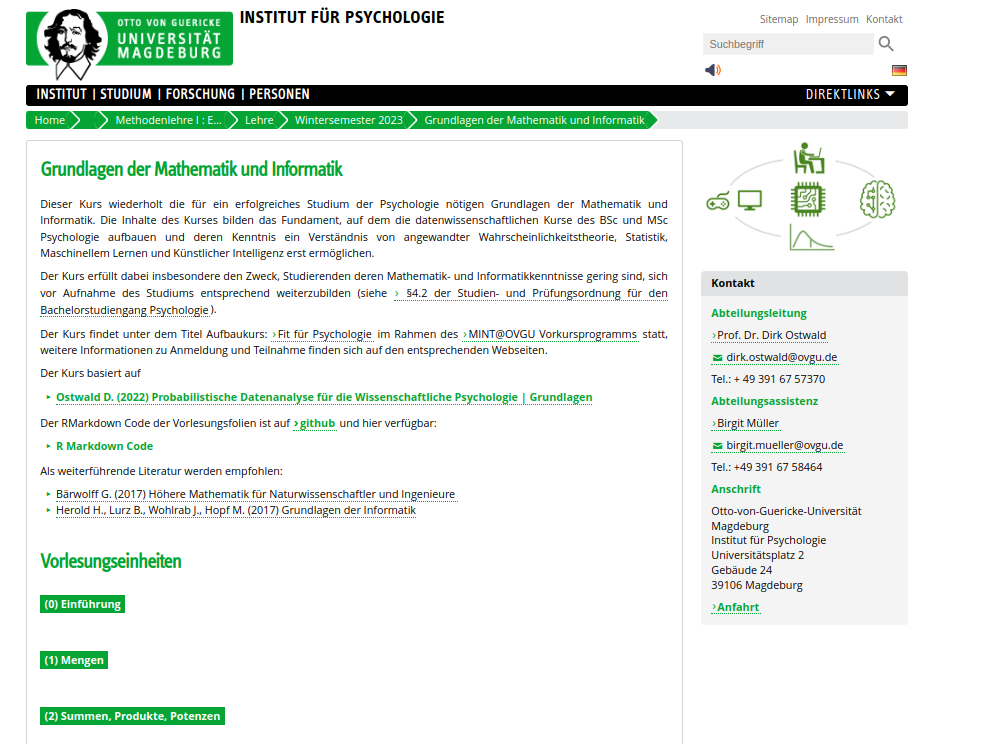
\includegraphics[width=0.75\linewidth]{../Abbildungen/glmi_0_kursseite} \end{center}
\color{red}{TODO: git einfügen?}
\end{frame}

\begin{frame}{Fit für Psychologie - Literaturempfehlungen}
\protect\hypertarget{fit-fuxfcr-psychologie---literaturempfehlungen}{}
\href{https://wasd.urz.uni-magdeburg.de/dostwald/}{\textcolor{blue}{Probabilistische Datenanalyse für die Wissenschaftliche Psychologie}}

\vspace{7mm}

\begin{center}
\includegraphics[width=0.8\linewidth]{../Abbildungen/glmi_0_pdwp} \end{center}
\end{frame}

\begin{frame}{Fit für Psychologie - Literaturempfehlungen}
\protect\hypertarget{fit-fuxfcr-psychologie---literaturempfehlungen-1}{}
\href{https://www.springer.com/de/book/9783662550212}{\textcolor{blue}{Bärwolff, G (2017) Höhere Mathematik}}

\vspace{5mm}

\begin{center}
\includegraphics[width=0.35\linewidth]{../Abbildungen/glmi_0_baerwolff} \end{center}
\end{frame}

\begin{frame}{Fit für Psychologie - Literaturempfehlungen}
\protect\hypertarget{fit-fuxfcr-psychologie---literaturempfehlungen-2}{}
\href{https://www.pearson.de/grundlagen-der-informatik-9783863268039}{\textcolor{blue}{Herold, H et al. (2017) Grundlagen der Informatik}}

\vspace{5mm}

\begin{center}
\includegraphics[width=0.35\linewidth]{../Abbildungen/glmi_0_herold} \end{center}
\end{frame}

\begin{frame}{Orga - Termine}
\protect\hypertarget{orga---termine}{}
\color{red}{TODO: kleinen Wochenplan erstellen?}
\end{frame}

\begin{frame}[plain]{}
\protect\hypertarget{section-2}{}
Q \& A
\end{frame}

\end{document}
